\graphicspath{ {./JiaweiZhuang/HW2_figures/bernoulli_question/} }

\begin{solution} 

We find that the term $\frac{1}{2} \rho u^2$ is orders of magnitude smaller than the pressure $p$. This is because the velocity $u$ is small (a result of the small Reynolds number). The pressure $p$ is almost constant (only 0.002\% perturbation) over the entire domain. This is demonstrated by Fig \ref{fig:ber_case1} and Fig \ref{fig:ber_case2}, where we can see that $\frac{1}{2} \rho u^2 + p \approx p$. The pressure $p$ is almost $0.166$ everywhere, and the velocity perturbation is negligible. In this case, the Bernoulli estimate almost just uses $p_0$ to approximate $p_i$. The relative error is less than 0.002\%.

\begin{figure}[H]
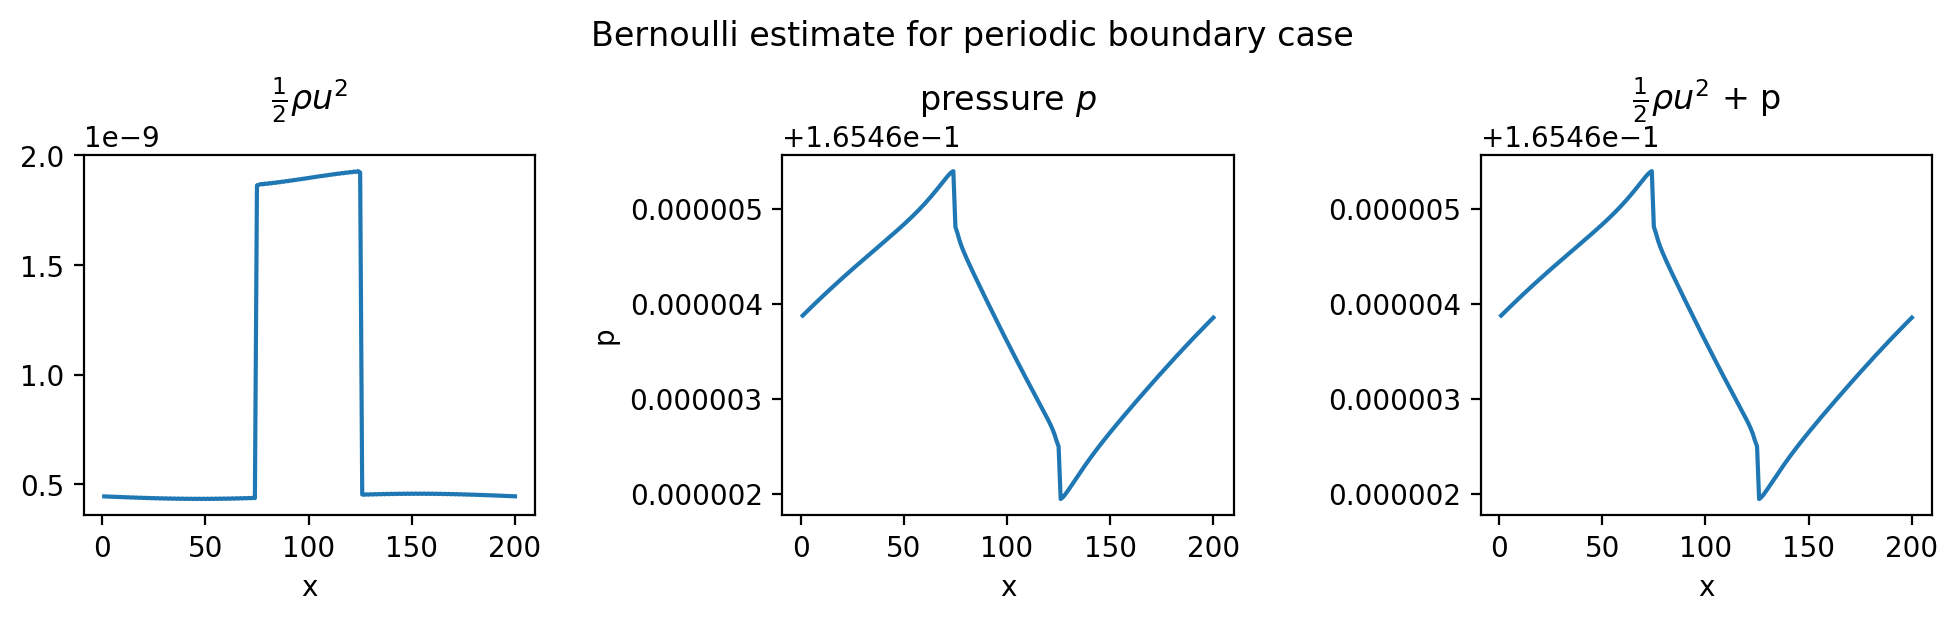
\includegraphics[scale=0.6]{bernoulli_case1_default}
\centering
\caption{Major quantities used in Bernoulli estimate, for periodic boundary case.}
\label{fig:ber_case1}
\end{figure}

\begin{figure}[H]
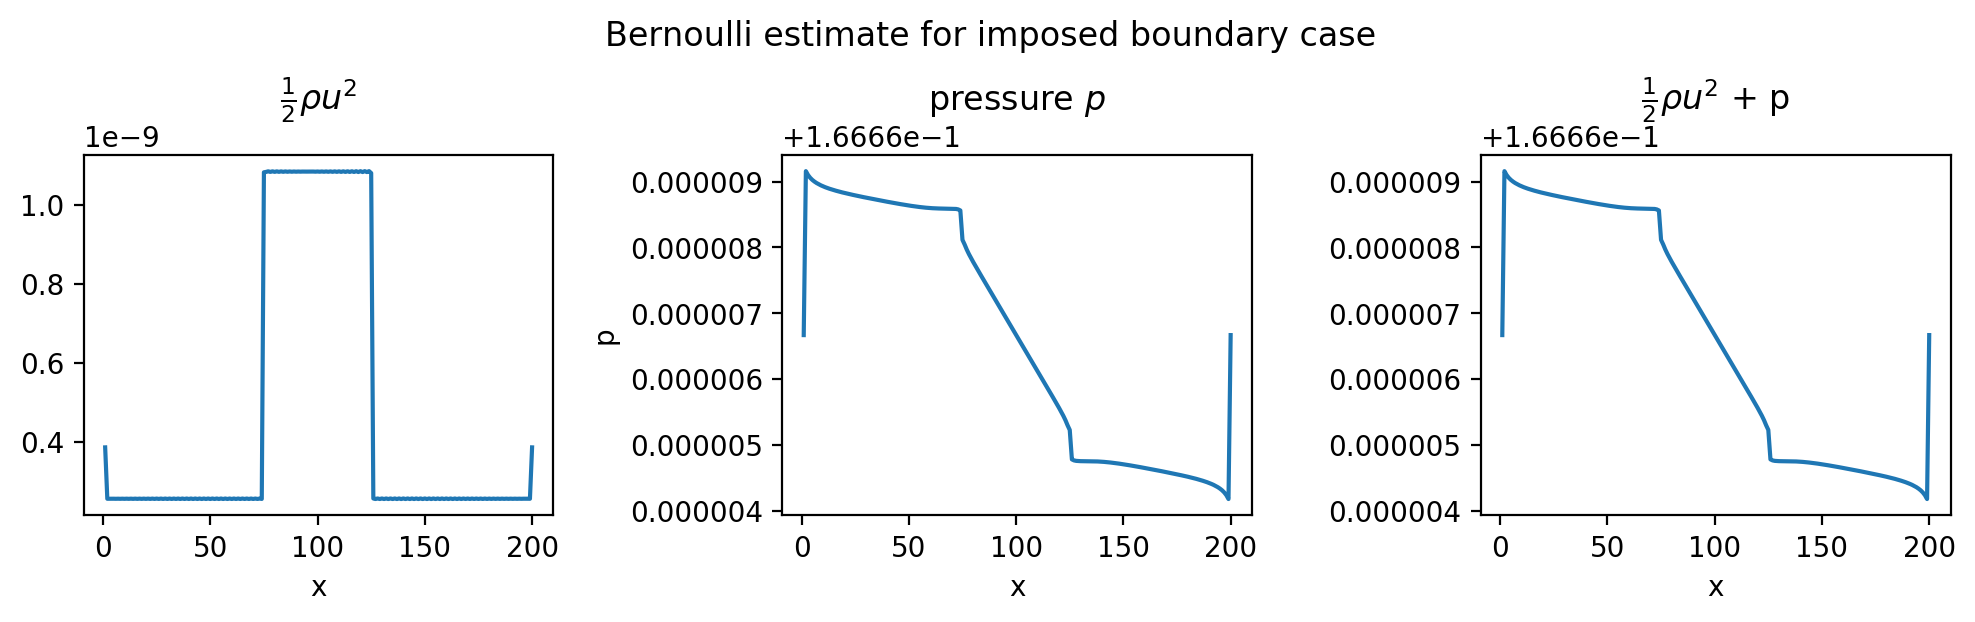
\includegraphics[scale=0.6]{bernoulli_case2_default}
\centering
\caption{Major quantities used in Bernoulli estimate, for non-periodic boundary case.}
\label{fig:ber_case2}
\end{figure}

\end{solution}


\begin{solution} 

Finally, we vary the LBM kinematic viscosity by tweaking the relaxation parameters $\Omega$. For all the previous cases we set $\Omega=1.0$, thus $\nu=1/6=0.1667$, which is the upper bound of $\nu$. For the lower bound $\nu=0.05$, the corresponding $\Omega = 1.54$. The velocity fields with different viscosity are shown in Fig \ref{fig:u_case1_nus}. Smaller viscosity leads to higher velocity magnitude, as expected.

\begin{figure}[H]
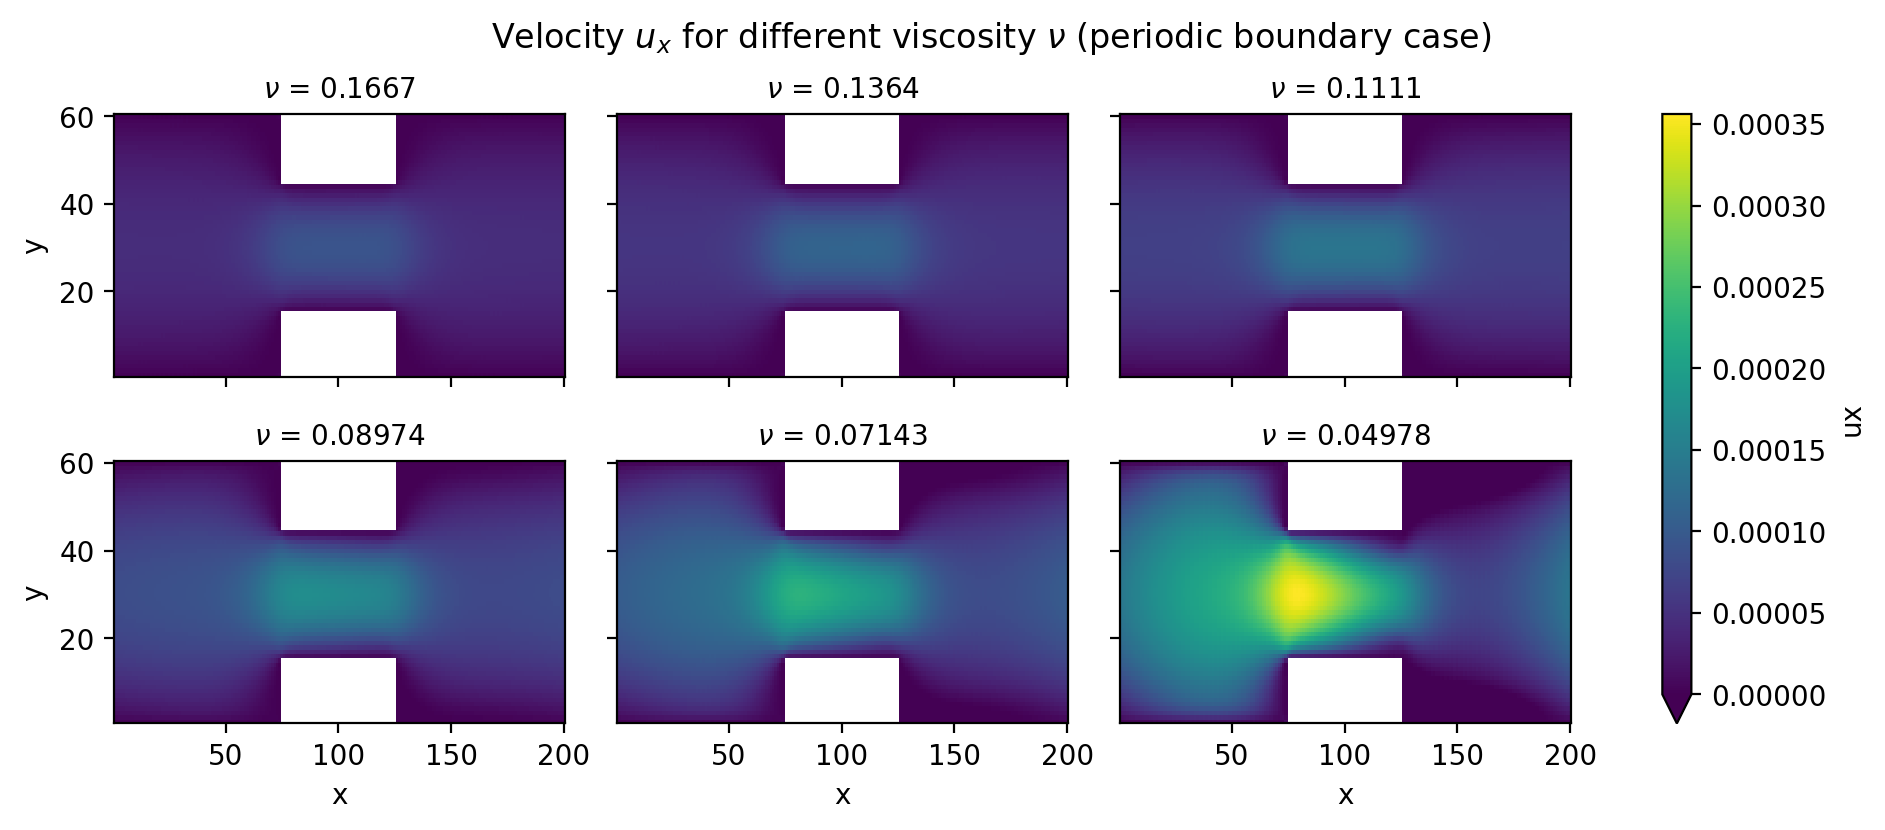
\includegraphics[scale=0.62]{u_case1_nus}
\centering
\caption{Velocity field for different viscosity $\nu$. Here uses Periodic boundary. The non-periodic one has similar behavior.}
\label{fig:u_case1_nus}
\end{figure}

For different viscosity $\nu$, the Bernoulli estimate has similar behavior, as shown in Fig \ref{fig:u_case1_nus}. The kinetic energy term $\frac{1}{2} \rho u^2$ becomes smaller with higher viscosity, as expected. The pressure term $p$, however, stays almost constant, and dominates the total term $\frac{1}{2} \rho u^2 + p$.

\begin{figure}[H]
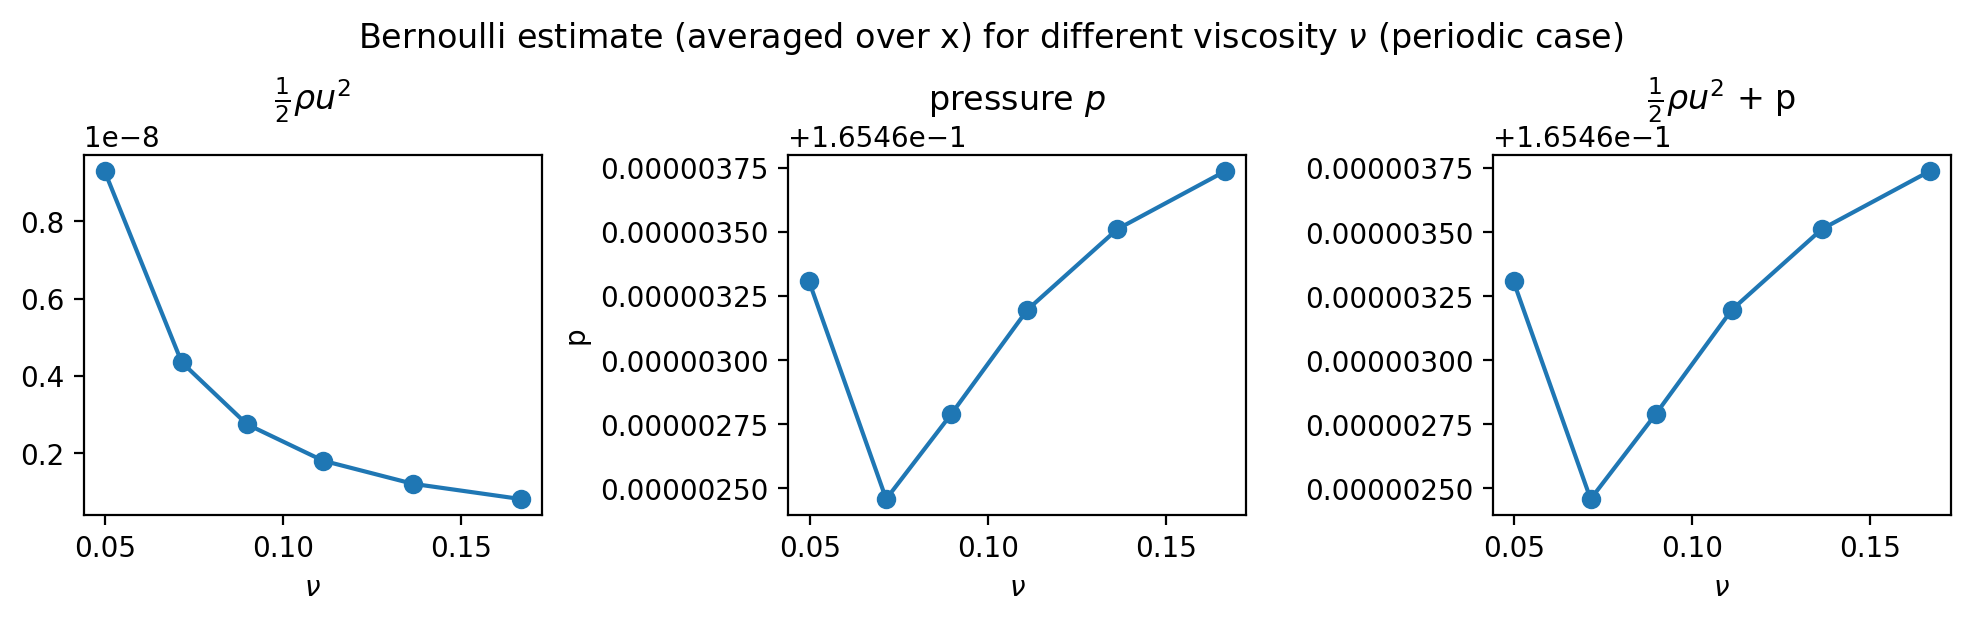
\includegraphics[scale=0.62]{bernoulli_case1_nus}
\centering
\caption{Major quantities used in Bernoulli estimate (averaged over x), for different viscosity $\nu$. Here uses Periodic boundary. The non-periodic one has similar behavior.}
\label{fig:bernoulli_case1_nus}
\end{figure}

\end{solution}


\begin{solution} 

All figures can generated by the Python notebook JiaweiZhuang/use\_LBM\_solver.ipynb.

\end{solution}